%声明文档类型和比例
\documentclass[aspectratio=169, 10pt, utf8, mathserif]{beamer}
%调用相关的宏包
\usepackage{amsmath, amsfonts}
\usepackage{graphicx}
\usepackage{subfigure}
\usepackage{multicol} %分栏
\usepackage{booktabs} %表格功能包
\usepackage{multirow} %合并多行表格
\usepackage{enumerate} %有序编号
\usepackage{listings} %代码包
\usepackage{xcolor} %代码高亮包
\lstset{
	language=Matlab, %代码语言使用的是matlab
	frame=shadowbox, %把代码用带有阴影的框圈起来
	rulesepcolor=\color{red!20!green!20!blue!20}, %代码块边框为淡青色
	keywordstyle=\color{blue}\bfseries, %代码关键字的颜色为蓝色,粗体
	commentstyle=\color{red}\textit, %设置代码注释的颜色
	showstringspaces=false, %不显示代码字符串中间的空格标记
	numbers=left, %显示行号
	numberstyle=\tiny, %行号字体
	stringstyle=\ttfamily, %代码字符串的特殊格式
	breaklines=true, %过长的代码自动换行
	extendedchars=false,  %解决代码跨页时,章节标题,页眉等汉字不显示的问题
	escapebegin=\begin{CJK*}{GBK}{hei},escapeend=\end{CJK*} %防止中文报错
	texcl=true}

\newtheorem{thm}{Theorem}
\newtheorem{defn}{Definition}
\newtheorem{conv}{Convention}
\newtheorem{prop}{Proposition}
\newtheorem{rem}{Remark}
\newtheorem{lem}{Lemma}
\newtheorem{cor}{Corollary}
\newtheorem{blk}{ }


\usetheme{Berlin} %主题包之一,直接换名字即可
\usefonttheme{professionalfonts}

% 设置用acrobat打开就会全屏显示
\hypersetup{pdfpagemode=FullScreen}

%--------------正文开始---------------
\begin{document}

%每个章节都有小目录
\AtBeginSection[]
{
 \begin{frame}<beamer>
   \tableofcontents[currentsection]
 \end{frame}
}

\title{Random Matrix
}
\subtitle{Spectrum estimation for large dimensional covariance matrices using random matrix theory}
\author{Yuheng Ma\hspace{3em}      
	Xinyi Wu \hspace{3em}
	Keyu Zhang}

\date{\today}
\begin{frame}
    %\maketitle
    \titlepage
\end{frame}

\begin{frame}
	\frametitle{Content}
	\tableofcontents[hideallsubsections]
\end{frame}

\section{Background introduction}
\subsection{Background introduction}
\begin{frame}
	\frametitle{Background introduction}
For i.i.d random vector $X_1\dots,X_n\in R^p$,and that the covariance of $X_i$ is $\Sigma_p$. We call X the data matrix whose rows are the $X_i$’s. How to estimate the eigenvalues of the population covariance matrix?

When p is fixed, n goes to $\infty$:

(Anderson,1963):Eigenvalues of the sample covariance matrix $S_p=(X-\overline{X})'(X-\overline{X})/(n-1)$ are good estimators of eigenvalues of $\Sigma_p$

 when comes to to “large n, large p”:
 
 For example, we consider p/n $\rightarrow$ r, $\Sigma_p=Id_p$, if $X_i$ i.i.d and have a forth moment, we know that \[l_1\rightarrow (1+\sqrt{r})^2 a.s.\]
\end{frame}
\subsection{Random Matrix}
\begin{frame}
	\frametitle{Random Matrix: From vectors to measures}
	
Suppose we have a vector $(y_1,\dots,y_p)$ in $R_p$. We can associate to it the following measure:\[dG_p(x)=\frac{1}{p}\sum_{i=1}^{p}\delta_{y_i}(x)\]

 We denote by $H_p$ the spectral distribution of the population covariance matrix $\Sigma_p$, i.e the measure associated with the vector of eigenvalues of $\Sigma_p$.
 
 Similarly, we denote by $F_p$ the measure associated with the eigenvalues of the sample covariance matrix $S_p$. 
\end{frame}
\begin{frame}
	\frametitle{Random Matrix: Convergence}
	Notion of convergence:  Weak convergence of probability measures.
	
	The \textbf{Stieltjes transform }of a measure G on R is defined as\[m_G(z)=\int\frac{dG(x)}{x-z}, z\in C^+\]
	
\textbf{Properties}: 	

If $G_n$ is a sequence of probability measures and $m_{Gn}(z)$ has a (pointwise) limit m(z) for all $z\in C^+$, then there exists a probability measure G with Stieltjes transform $m_G = m$ if and only if $\lim_{y\rightarrow\infty}-iym(iy) = 1$. If it is the case, $G_n$ converges weakly to G. 
\end{frame}
\begin{frame}
	\frametitle{Random Matrix: the Mar\v{c}enko-Pastur equation}
	  X:n×p data matrix.  $S_p = X'X/n$   $H_p$: the population spectral distribution
	  
	 ${m_{F_p}}$ :the Stieltjes transform of the spectral distribution, $F_p$, of $S_p$. 
	   
	 ${v_{F_p}(z)=(1-p/n)\frac{-1}{z}+\frac{p}{n}m_{F_p}(z)}$,which is actually the Stieltjes transform of the spectral distribution $XX'/n$
	 
	\begin{thm}

	 
	  Suppose the data matrix X can be written $X=Y\Sigma_p^{\frac{1}{2}}$ , where  $\Sigma_p$ is a p×p positive definite matrix and Y is an n×p matrix whose entries are i.i.d (real or complex), with $E(Y_{i,j}) = 0$, $E(|Y_{i,j}|^2) = 1$ and $E(|Y_{i,j}|^4)<\infty$. Assume that $H_p$ converges weakly to a limit denoted $H_\infty$.
	  	\end{thm}
\end{frame}
\begin{frame}
	\frametitle{Random Matrix: the Mar\v{c}enko-Pastur equation}
		\begin{blk}
	Then, when $p,n\rightarrow$, and $p/n\rightarrow r$, $r\in(0,\infty)$ ,
	
	1.$v_{F_p}(z)\rightarrow v_\infty(z)$ a.s, where $v_\infty(z)$ is a deterministic function.
	
	2. $v_\infty(z)$ satisfies the equation \[-\frac{1}{v_\infty(z)}=z-r\int\frac{\lambda dH_\infty(\lambda)}{1+\lambda v_\infty(z)},\forall z\in C^+\]
	
	3. The previous equation has one and only one solution which is the Stieltjes transform of a measure.
	\end{blk}
	 
\end{frame}
\section{Algorithm}

\begin{frame}
	\frametitle{Formulation of the estimation problem}
\textbf{Goal}: 

estimate the population eigenvalues

\textbf{Strategy}:

1. use the Mar\v{c}enko-Pastur equation to estimate the measure $H_\infty$.($\hat{H}$)

2. estimate $\lambda_i$ as the i-th quantile of our estimated distribution $\hat{H}_\infty$.

\textbf{Fact}:

since we are considering fixed distribution asymptotics, our estimate of $H_\infty$ will serve as our estimate of $H_p$, so  $\hat{H}_\infty=\hat{H_p}$.


\end{frame}
\begin{frame}
	\frametitle{Formulation of the estimation problem}
	\[-\frac{1}{v_\infty(z)}=z-r\int\frac{\lambda dH_\infty(\lambda)}{1+\lambda v_\infty(z)},\forall z\in C^+\]
	
	\textbf{Step 1}:Estiamte $H_\infty$ from $F_p$.
	
	Compute eigenvalue of $S_p$ $\rightarrow$ $F_p$ $\rightarrow$ $v_{F_p}(z)$ $\stackrel{ \{z_j\}_{j=1}^{J_n}}{\longrightarrow}$ $\{v_{F_p}(z_j)\}_{j=1}^{J_n}$
	
	\[\hat{H}_\infty=\mathop{\arg\min}_{H} L(\{\frac{1}{v_{F_p}(z_j)}+z_j-\frac{p}{n}\int\frac{\lambda dH(\lambda)}{1+\lambda v_{F_p}(z_j)}\}_{j=1}^{J_n})\]
\end{frame}
\begin{frame}
	\frametitle{Discretization}
	\textbf{Step 2}:Discretization.
	
	Naturally, dH can be simply approximated by a weighted sum of point masses:\[dH(x)\approx\sum_{k=i}^{K}w_k\delta_{t_k}(x)\]
	
	where $\{t_k\}_{k=1}^{K}$ is a grid of points, chosen by us, and $w_k$’s are weights, which satisfies \[\sum_{k=1}^{K}w_k=1,w_k\geq0\] 
	
\end{frame}
\begin{frame}
	\frametitle{Discretization}
	Hence finding a measure that approximately satisfies Equation (M-P) is equivalent to finding a set of weights $\{w_k\}_{k=1}^{K}$,for which we have
		\[-\frac{1}{v_{F_\infty}(z_j)}\approx z_j-\frac{p}{n}\sum_{k=1}^{K}\frac{w_{k}t_k}{1+t_{k}v_{F_\infty}(z_j)},\forall j\]
	
	 Replace $v_\infty$ by $v_{F_p}$. Our problem is thus to find $\{w_k\}_{k=1}^{K}$ such taht,
	\[-\frac{1}{v_{F_p}(z_j)}\approx z_j-\frac{p}{n}\sum_{k=1}^{K}\frac{w_{k}t_k}{1+t_{k}v_{F_p}(z_j)},\forall j\]
\end{frame}
\begin{frame}
	\frametitle{Convex Optimization formulation}
	\textbf{Approximation errors}
	\[e_j=\frac{1}{v_{F_p}(z_j)}+z_j-\frac{p}{n}\sum_{k=1}^{K}\frac{w_{k}t_k}{1+t_{k}v_{F_p}(z_j)}\]
	
\textbf{Step 3}:Formulating our problem as a convex optimization problem.

 “$L_\infty$” version: Find $w_k$’s to\[Minimize\max_{j=1,\dots,J_n}max\{|Re(e_j)|,|Im(e_j)|\}\]
\end{frame}
\begin{frame}
	\frametitle{Convex Optimization formulation}
 The “translation” of the problem into a convex optimization problem is\[\min_{(w_1,\dots,w_K,u)}u\]\[\forall j,-u\leq Re(e_j)\leq u\]\[\forall j,-u\leq Im(e_j)\leq u\]\[\sum_{k=1}^{K}w_k=1\]\[w_k\geq0,\forall j\]

\end{frame}


\section{Consistency}

\begin{frame}
	\frametitle{Consistency}
	Our estimate is consistent in $L^{\infty}$ sense. The general result is as follows.\\
		\begin{thm} 
	 Under setups in previous thm, $H_p\Rightarrow H_{\infty}$ and $\frac{p}{n}\to \gamma$. $J_1 \cdots \in \mathbb{Z}$ with limit $\infty$ and $z_1,\cdots\in \mathbb{C}^+$ bounded and convergent, $\hat{H}_p$ is the solution to 
	 $$
	 \widehat{H}_{p}=\underset{H}{\arg \min } \max _{j \leq J_{n}}\left|\frac{1}{v_{F_{p}}\left(z_{j}\right)}+z_{j}-\frac{p}{n} \int \frac{\lambda d H(\lambda)}{1+\lambda v_{F_{p}}\left(z_{j}\right)}\right|
	 $$
	 Then 
	 $$
	 \hat{H}_p\Rightarrow H_{\infty} \;\;\;\;\; a.s.
	 $$
	 \end{thm}
	Same thing holds for our estimation which is made over a mixture of diracs. 
\end{frame}

\begin{frame}
	\frametitle{Idea of Proof}
	$$\Delta =\frac{1}{v_{F_{p}}\left(z_{j}\right)}+z_{j}-\frac{p}{n} \int \frac{\lambda d H(\lambda)}{1+\lambda v_{F_{p}}\left(z_{j}\right)}$$
	Recall Thm1, when $H_p\Rightarrow H_{\infty}$
	\begin{itemize}
	\item $v_{F_p}\to v_{\infty}$ a.s. (Thm 1)
	\item $v_{F_p}\to v_{\infty}$ uniformly (Prop 1)
	\item $Im(v_{F_p})$ bounded away from 0 (Prop 2)
	\item $|\Delta|\downarrow0$ (Prop 3)
	\item $\hat{H}_p\Rightarrow H_{\infty}$ (Lemma)
	\item $\hat{H}_p$ is fine to be sum of atoms (Cor)
	\end{itemize}
\end{frame}
\begin{frame}
	\frametitle{Lemma}
	Find convergent $\hat{H}_p$ over constraint over convergent sequence of $z_i$.\\
	\begin{lem}
	With $\epsilon_n \downarrow 0$ and $$
	\forall j \leq J_{n} \quad\left|\frac{1}{v_{F_{p}}\left(z_{j}\right)}+z_{j}-\frac{p}{n} \int \frac{\lambda d \tilde{H}_{p}(\lambda)}{1+\lambda v_{F_{p}}\left(z_{j}\right)}\right|<\varepsilon_{n}
	$$
	Also, $v_{F_p}(z_j)\to v_{\infty}(z_j) $ and both analytic as well as bounded away from reals, then we have convergence of $\tilde{H}_{p}(\lambda)$ to $H_{\infty}$.
	\end{lem}
\end{frame}

\begin{frame}
	\frametitle{Proposition}
	\begin{prop}
	Stieltjes transform $S_H$ is Lipschitz by $\frac{1}{u_{min}^2}$ on $\mathbb{C}^+\cap\{Im(z)>u_{min}\}$
	\end{prop}
	\begin{prop}
	Population spectral distribution $H_p$ has a limit $H_{\infty}$, where all spectra uniformly bounded, then for a ball in $\mathbb{C}^+$, 
	$$
	\exists N \quad n>N \quad \Rightarrow \quad \inf _{n, z \in B\left(z_{0}, r\right)} \operatorname{Im}\left(v_{F_{p}}(z)\right)=\delta>0
	$$
	where $v_{F_p}$ is the Stieltjes transform of $F_p$.
	\end{prop}
\end{frame}


\begin{frame}
\frametitle{Proposition}
\begin{prop}
If $\exists$ N s.t. any n>N, $|v_{F_p}(z)-v_{\infty}(z)|<\epsilon$, and $|Im(v_{\infty}(z))|>u_{min}$, then 
for $
\epsilon<\frac{u_{min}}{2},\exists N^{\prime} \in \mathbb{N}, \forall z \in B\left(z_{0}, r\right), \forall n>N^{\prime}
$.
$$
\left|\frac{1}{v_{F_{p}}(z)}+z-\frac{p}{n} \int \frac{\lambda d H_{\infty}(\lambda)}{1+\lambda v_{F_{p}}(z)}\right|<2 \varepsilon \frac{1+2 \gamma}{u_{\min }^{2}}
$$
\end{prop}
\end{frame}
\begin{frame}
	\frametitle{Consistency of Proposed Algorithm}
	Only need to show Proposition 3 holds for sum of atoms.
	\begin{cor}
	Restrict $\hat{H}_p$  over measures which are sums of atoms, the locations of which are restricted to belong to a grid (depending on n) whose step size is going to 0 as $n\to \infty$. Then everything holds.
\end{cor} 
\end{frame}


\section{Simulations}

\begin{frame}
	\frametitle{Simulations}
	\textbf{Case 1}:Identity covariance:$\Sigma$=Id
	
	\vspace*{ 0.7cm }
	\textbf{Case 2}:“Two spike” spectrum: $\Sigma$ has d/2 eigenvalues equal to 1 and d/2 equal to 2
	
		\vspace*{ 0.7cm }
\textbf{Case 2}:covariance $\Sigma= T$ where
$T_{i,j}= 0.3^{\vert i-j\vert}$is a d×d Toeplitz matrix
\end{frame}

\begin{frame}
\frametitle{eigenvalues of sample covarience matrix}
\begin{figure}[htbp]
	\subfigure[Case1]{
		
\includegraphics[scale=0.13]{1.jpg}}
	\quad
	\subfigure[Case2]{
	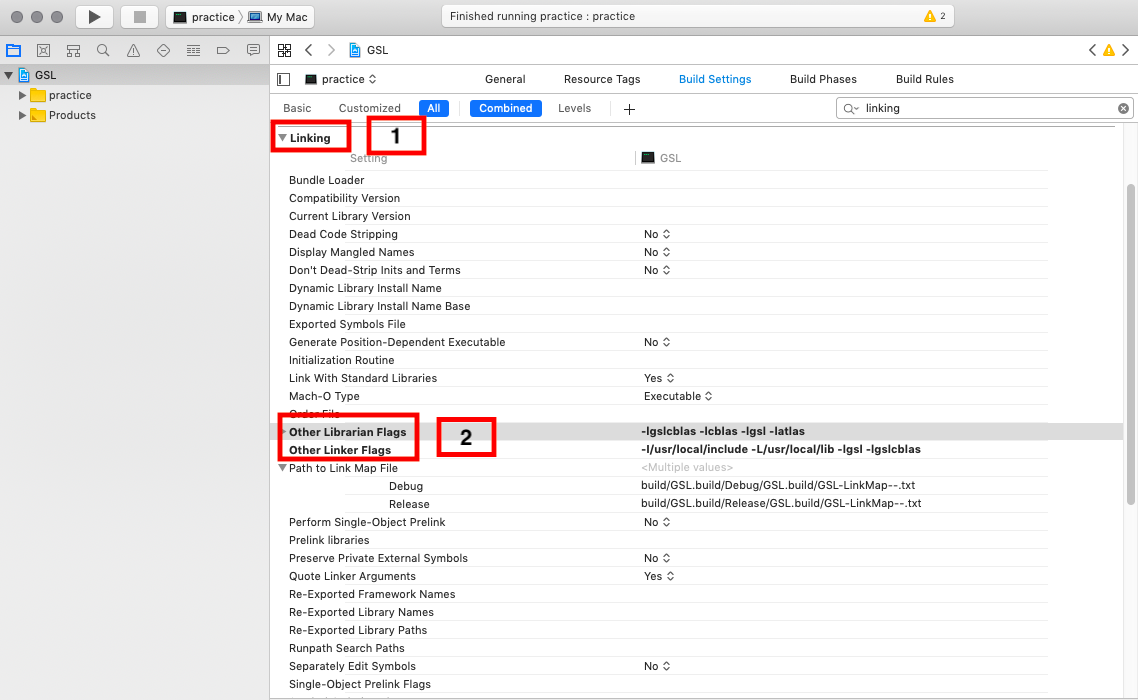
\includegraphics[scale=0.13]{2.jpg}}
\quad
	\subfigure[Case3]{
	\includegraphics[scale=0.13]{15.jpg}}
\quad
\end{figure}

\end{frame}

\begin{frame}
\frametitle{Case1}
\begin{figure}[htbp]
	\subfigure[n=500,p=100]{
		
\includegraphics[scale=0.17]{3.jpg}}
	\quad
	\subfigure[n=500,p=250]{
		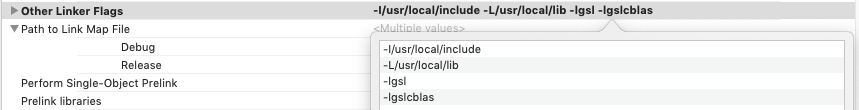
\includegraphics[scale=0.17]{4.jpg}}
	\quad

\end{figure}

\end{frame}

\begin{frame}
\frametitle{Case1}
\begin{figure}[htbp]
	\subfigure[n=500,p=500]{
		\includegraphics[scale=0.17]{5.jpg}}
	\quad
	\subfigure[n=500,p=1000]{
		\includegraphics[scale=0.17]{6.jpg}}
	\quad
	
\end{figure}

\end{frame}

\begin{frame}
\frametitle{Case2}
\begin{figure}[htbp]
	\subfigure[n=500,p=100]{
		\includegraphics[scale=0.17]{7.jpg}}
	\quad
	\subfigure[n=500,p=250]{
		\includegraphics[scale=0.17]{8.jpg}}
	\quad

	
\end{figure}

\end{frame}

\begin{frame}
\frametitle{Case2}
\begin{figure}[htbp]
			\subfigure[n=500,p=500]{
		\includegraphics[scale=0.17]{9.jpg}}
	\quad
	\subfigure[n=500,p=1000]{
		\includegraphics[scale=0.17]{10.jpg}}
	\quad


\end{figure}

\end{frame}

\begin{frame}
\frametitle{Case3}
\begin{figure}[htbp]
	\subfigure[n=500,p=100]{
		\includegraphics[scale=0.17]{11.jpg}}
	\quad
	\subfigure[n=500,p=250]{
		\includegraphics[scale=0.17]{12.jpg}}
	\quad
	
	
\end{figure}

\end{frame}

\begin{frame}
\frametitle{Case3}
\begin{figure}[htbp]
	\subfigure[n=500,p=500]{
		\includegraphics[scale=0.17]{13.jpg}}
	\quad
	\subfigure[n=500,p=1000]{
		\includegraphics[scale=0.17]{14.jpg}}
	\quad
	
	
\end{figure}

\end{frame}

\section{Conclusion}

\begin{frame}
	\frametitle{Conclusion}
	
\end{frame}


\begin{frame}
	\centering{Thanks for watching}
\end{frame}

\end{document}